\section*{Aufgabe 1}
\subsection*{1a)}
Zunächst soll der Ausdruck für die eindimensionale Zustandssumme $Z$ für das
Ising-Modell (Hamiltonian s. Skript) mit nicht verschwindendem Magnetfeld hergeleitet werden. Diese ist
nach dem Skript, Gl. (8.14), zu bestimmen als
\begin{eqnarray}
Z &=& \mathrm{Tr}\left[T^L\right]\\
\mathrm{mit\quad} T_{σσ'} &=& \exp[βσσ' + βB(σ+σ')/2]
\end{eqnarray}
σ und $σ'$ können hierbei $\pm 1$ sein. Damit ergibt sich die folgende Matrix $T$:
\begin{eqnarray}
T = \begin{pmatrix} e^{β(1+B)} & e^{-β} \\ e^{-β} & e^{β(1-B)} \end{pmatrix}
\end{eqnarray}

Nun sind die Eigenwerte dieser Matrix zu berechnen, um eine Diagonalform herstellen zu können,
mit dem Ziel, die Potenzierung der Matrix möglichst einfach werden zu lassen. Dies wird in den folgenden
Zeilen getan.

\begin{eqnarray}
0 &=& \det[T-λ] = (e^{β(1+B)}-λ)(e^{β(1-B)}-λ) - e^{-2β}\\
&=& λ^2 - λe^β\underbrace{\left(e^{βB} + e^{-βB}\right)}_{2\cosh(βB)} + \underbrace{e^{2β} - e^{-2β}}_{2\sinh(2β)}\\
→ λ_{\pm} &=& e^β\cosh(βB) \pm \sqrt{e^{2β}\cosh^2(βB) - 2\sinh(2β)}
\end{eqnarray}

Damit lässt sich die Potenzierung und anschließende Spurbildung der Matrix leicht
analytisch durchführen:
\begin{eqnarray}
\mathrm{Tr}[T^L] = λ_+^L + λ_-^L
\end{eqnarray}

$Z$ ist somit exakt bekannt. Um nun den Grenzwert $L→∞$ durchzuführen, wird ausgenutzt,
dass $λ_-$ kleiner als $λ_+$ ist. Daher ist der Beitrag von $λ_-$ im Grenzfall
vernachlässigbar.

\begin{eqnarray}
Z \approx λ_+^L = \left(e^β\cosh(βB) + \sqrt{e^{2β}\cosh^2(βB) - 2\sinh(2β)}\right)^L
\end{eqnarray}

\subsection*{1b)}
Hier soll aus der bekannten, kanonischen Zustandssumme die mittlere Energie und
Magnetisierung berechnet werden. Dafür wird die Relation aus Skript, Gl. (8.9) (mittlere
Energie) und Gl. (8.10) (mittlere Magnetisierung) verwendet. Die Relation für die mittlere
Energie $E$ lautet wie folgt:
\begin{eqnarray}
E &=& \langle H \rangle = -\frac{∂\ln Z}{∂β}\\
&=& {{\left({{2e^{2β}B\cosh \left(βB\right)\sinh \left(βB\right)+2e^{2β}\cosh^2
 \left(βB\right)-4\cosh \left(2β\right)}\over{2\sqrt{
 e^{2β}\cosh ^2\left(βB\right)-2\sinh \left(2β\right)}}}+e^β(B\sinh \left(βB\right)+
 \cosh \left(βB\right))\right)L}
 \over{\sqrt{e^{2β} \cosh^2\left(βB\right)-2\sinh \left(2β\right)}+e^{
 β}\cosh \left(βB\right)}}
\end{eqnarray}

Für die Magnetisierung $M$ ergibt sich folgendes:
\begin{eqnarray}
\langle M \rangle &=& \frac{1}{β}\frac{∂\ln Z}{∂B}\\
&=& {L\left({{e^{2β}\cosh \left(βB\right)\sinh \left(βB\right)}\over{\sqrt{e^{2β}\cosh^2
 \left(βB\right)-2\sinh \left(2β\right)}}}+e^β \sinh \left(βB\right)\right)}
 \over{\sqrt{e^{2β}\cosh ^2\left(βB\right)-2\sinh \left(2β\right)}+e^{β}\cosh \left(βB\right)}
\end{eqnarray}

\subsection*{1c}

Schließlich war die Magnetisierung in Abhängigkeit von β und $B$ zu plotten.
Dafür wurde das in \lref{plot_mag} dargestellte Skript geschrieben.

\lstinputlisting[label=lst:plot_mag,caption={magnetisierung.m}]{../code/magnetisierung.m}

Die daraus erstellte Graphik ist in \fref{magnetisierung} dargestellt.

\begin{figure}[htb]
  \centering
  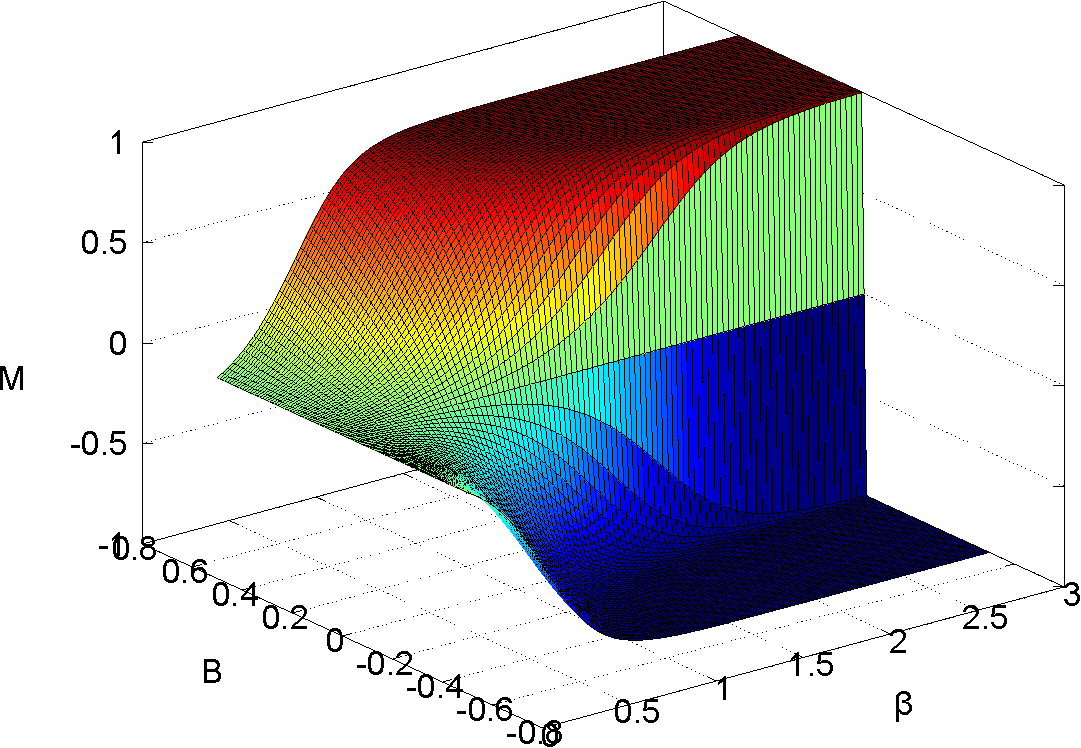
\includegraphics[width=0.8\columnwidth,keepaspectratio]{../tmp/magnetisierung-crop}
  \caption{Magnetisierung in Abhängigkeit von β und $B$, jeweils in natürlichen Einheiten}
  \label{fig:magnetisierung}
\end{figure}

Das Ergebnis entspricht den Erwartungen, da bei großen Magnetfeldern die Magnetisierung
ihren positiven oder negativen Grenzwert anstrebt, je nach Ausrichtung des Magnetfelds.
Weiterhin ist zu beobachten, dass bei kleinen Temperaturen, also großen β-Werten,
die Magnetisierung fast sofort ihren Grenzwert erreicht, während bei großen Temperaturen,
also kleinen β-Werten, auch große äußere Magnetfelder die Magnetisierung nicht 
wesentlich vom Wert $M=0$ abweichen lassen. Dies entspricht der Vorstellung, dass
eine hohe Temperatur die einzelnen Spins stärker aus der Ausrichtung in eine
Richtung ablenkt als eine geringe Temperatur.

\section*{Aufgabe 2)}

In der zweiten Aufgabe wurde ein ein- und ein zweidimensionales Spin-Gitter untersucht.
Dabei sollten diese Gitter jeweils einmal geordnet und einmal ungeordnet, also
zufällig belegt sein. Für alle Fälle war die Magnetisierung und die Energie zu messen.
Die Randbedingungen waren periodisch.

Der Code, der diese Aufgabenstellung bearbeitet, ist in \lref{main} dargestellt.

\lstinputlisting[label=lst:main,caption={main.cpp}]{../code/main.cpp}

Als Zufallszahlengenerator wurde die in der ROOT-Klasse \texttt{TRandom3} zur
Verfügung gestellte Funktion \texttt{Uniform} verwendet, die gleichverteilte Zufallszahlen
generiert.

Weiterhin wurde immer überprüft, welche Indizes die Nachbarn des Koordinatenursprungs haben,
um die korrekte Implementierung der Randbedingungen zu testen.

Das Programm wurde mit verschiedenen Parametern aufgerufen, um die einzelnen
Konfigurationen zu testen, wobei der folgende Output resultierte:

\begin{lstlisting}[caption=Aufruf und Output von \lref{main},label=lst:output]
$> ./main 10 1 0
magnetization: 0.4
energy: 10
neighbours of (0,0,...):
  1
  9
$> ./main 10 1 1
magnetization: 1
energy: 40
neighbours of (0,0,...):
  1
  9
$> ./main 10 2 0
magnetization: 0.46
energy: 176
neighbours of (0,0,...):
  1
  10
  9
  90
$> ./main 10 2 1
magnetization: 1
energy: 600
neighbours of (0,0,...):
  1
  10
  9
  90
\end{lstlisting}
Unabhängig von der Dimension ist demnach die Energie und die Magnetisierung für
geordnete Systeme deutlich größer als für ungeordnete Systeme, was zu erwarten
war. Auch die Überprüfung der Nachbarn stimmt mit den Erwartungen überein. 